%!TEX root = ../thesis.tex
%!TEX root = ../thesis.tex

\newcommand{\vrms}{\text{v}_\text{n}^\text{rms}}
\newcommand{\vsq}{\overline{\text{v}_\text{n}^2}}
\newcommand{\vn}{\text{v}_\text{n}}
\newcommand{\vin}{\text{v}_\text{in}}
\newcommand{\vout}{\text{v}_\text{out}}
\newcommand{\Sin}{\text{S}_{\vn}^\text{in}}
\newcommand{\Sout}{\text{S}_{\vn}^\text{out}}
\newcommand{\Svn}{\text{S}_{\vn}}


\chapter{Noise}
\label{ch:noise}
% TODO: Left to find out:
% Is the power to V_in conversion correct?

When performing measurements one is faced with the reality that no component is ideal. When a signal passes through the different parts of a set-up, noise is constantly being added. Noise is the term given for all the random fluctuations that are added to the signal. These fluctuations are the cumulative result of several noise source contributions.

Thermal noise is one of the most common sources of noise. It is the result of the random thermal fluctuations of electrons. It is an example of frequency-independent noise, also known as white noise. Noise sources can also be frequency-dependent, such as TLS, as discussed in Chapter~\ref{part:DRIE}. This is an example of $1/f$-noise: the amount of noise added increases with decreasing frequency. In fact, truly frequency-independent noise does not exist, as even white noise has been observed to decrease at extremely high frequencies (\SI{\sim e15}{\hertz}). At these frequencies a quantum correction needs to be added \cite[p50]{vasilescu2006electronic}.

When performing measurements one important question to ask is how much noise is being contributed to the signal. In this chapter a model is presented for the general set-up used for measuring superconducting resonators and qubits. Using this model it is possible to characterize the amount of noise by determining its associated noise temperature. Finally, this model is applied to the set-up used to characterize the resonators presented in Chapter~\ref{part:DRIE}.

\section{Characterizing noise}

\subsection{Circuit representations}


\begin{figure}[h]
    \centering
    \begin{subfigure}[b]{.43\textwidth}
        \includegraphics[width=\textwidth]{Figures/Noise/thevenin.png}%\figureinset{(a)}{2.55}{1.5}
        \caption{Th\'evenin representation}
        \label{fig:thevenin}
    \end{subfigure}
    \begin{subfigure}[b]{.49\textwidth}
        \includegraphics[width=\textwidth]{Figures/Noise/norton.png}%\figureinset{(b)}{2.55}{1.5}
        \caption{Norton representation}
        \label{fig:norton}
    \end{subfigure}
    \caption{Two equivalent representations of a system containing noise. Panel~\textbf{(a)} shows the Th\'evenin representation, in which a noiseless voltage source is connected in series with a noise voltage source. Panel~\textbf{(b)} shows the Norton representation, in which a noiseless current source is connected in parallel with a noise current source.}
\end{figure}

There are two circuit representations in which we can depict a system with a noise contribution: The Th\'evenin representation, and the Norton representation. In the Th\'evenin representation we can model the system as a voltage source, and the noise added to the system is a noise voltage source connected in series. In the Norton representation the system is a current source and the noise added is a noise current source connected in parallel to the current source. These two representations are identical and can be converted to each other. In this section we will adopt the Thev\'enin representation, and so the signal will be a voltage source combined in series with a noise voltage source.

Assuming the signal to be at a fixed frequency $\omega$ and amplitude $A$, the combined voltage $v(t)$ is then given by:

\begin{equation}
    \text{v}(t) = \text{v}_\text{signal}(t) + \text{v}_\text{noise}(t) = A \cos{\omega t} + \vn(t)
\end{equation}

Note that the mean value of the noise voltage $\overline{\vn}$ is equal to zero. The amount of noise can be quantified by the root-mean square noise voltage $\vrms$:
\begin{equation}
    \vrms = \sqrt{\overline{\text{v}^2} - \overline{\text{v}}^2} = \sqrt{\vsq}
    \label{eqn:v_rms}
\end{equation}

\subsection{Noise power spectral density}

One way of quantifying the noise of the system is through the noise power spectral density $S(f)$, which is the distribution of noise power per unit bandwidth as a function of frequency. For the Th\'evenin representation, the noise spectral density is defined in terms of voltage. When the only noise in the system is white noise, the spectral density is independent of frequency. It is then given by:

\begin{equation}
    S = \frac{\vsq}{\Delta f}
    \tagaddtext{[\si[per-mode=symbol]{\volt \squared \per \hertz}]}
    \label{eqn:noise spectral density definition}
\end{equation}

In this equation $\Delta f$ is the noise bandwidth. This is the bandwidth over which the noise is measured.

\newpage
\section{The model}

\begin{figure}
    \centering
    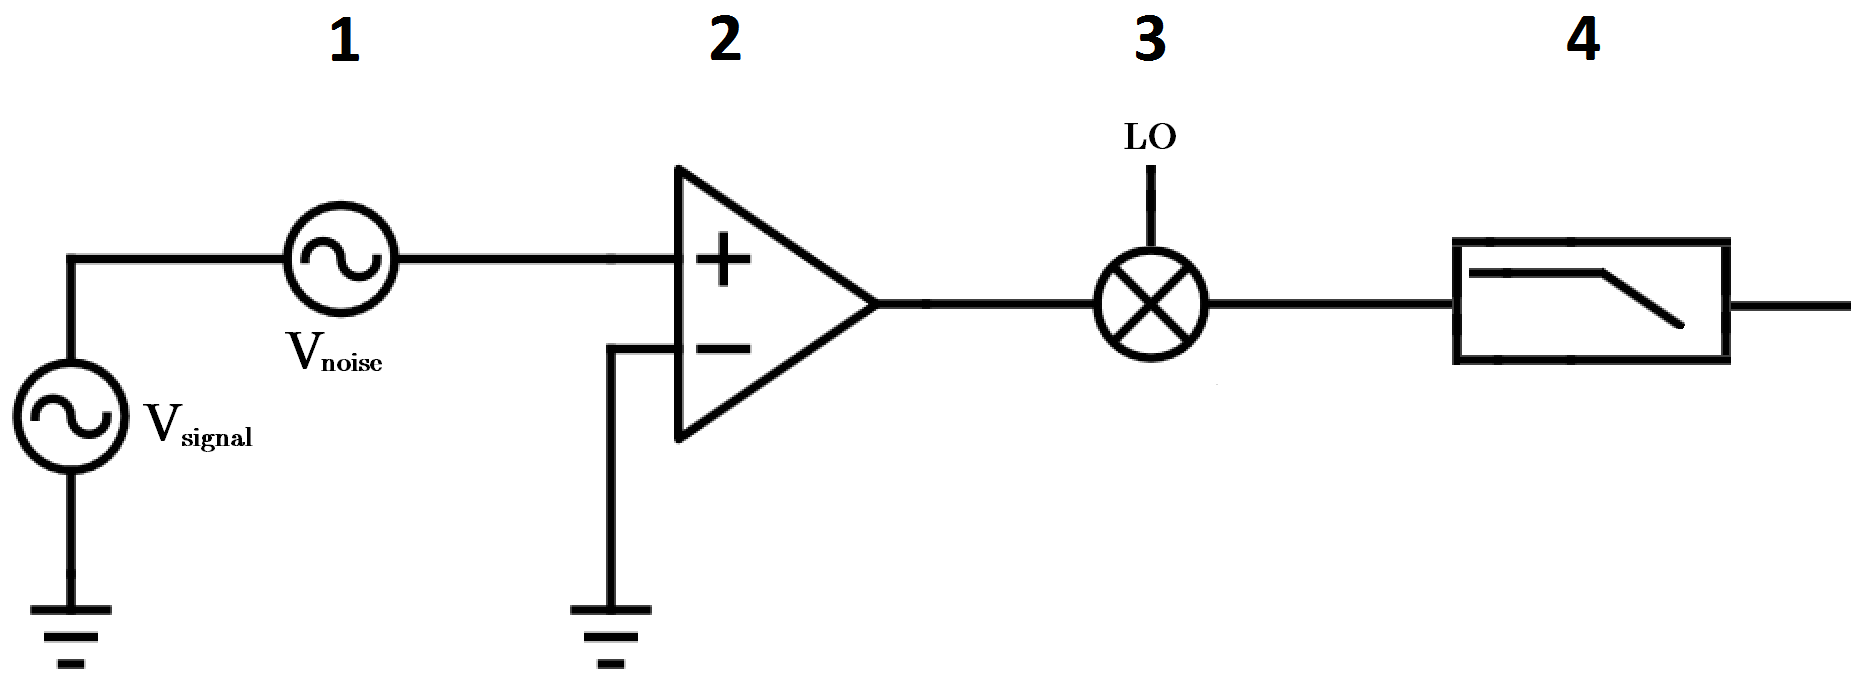
\includegraphics[width=.8\textwidth]{Figures/Noise/Noise model.png}
    \caption{Schematic representation of the measurement set-up including a noise source.}
    \label{fig:noise model}
\end{figure}


As shown in the schematic in Figure~\ref{fig:noise model}, we can model our set-up as a combination of four elements:

\begin{enumerate}
    \item A noise source.
    \item An amplifier to amplify the weak signal exiting the fridge.
    \item A mixer to downconvert the signal.
    \item A low-pass filter to remove unwanted high-frequency signal.
\end{enumerate}



\subsection{Noise source}

Using the Th\'evenin model, we can approximate the components up to the first amplifier in the fridge as a voltage source, with a noise voltage source connected in series.

We can include the noise added by the amplifier in the noise voltage source, in which case we assume the amplifier to be ideal. Furthermore, we assume the signal to be amplified sufficiently, such that the mixer and low-pass filter add a negligible amount of noise. We also ignore effect such as mixer leakage. With these assumptions all of the noise is originated from the noise voltage source.

We can associate an effective noise temperature to the noise voltage source. The noise temperature is defined as the temperature at which a resistor would produce an equal amount of noise. Note that, since we are comparing the system to a resistor, the noise needs to have an (approximately) white spectrum.

According to Nyquist's theorem \cite[p47]{vasilescu2006electronic}, if the system experiences white noise, and is in thermal equilibrium, the root-mean square noise voltage $\vrms$ is given by:

\begin{equation}
    \vrms = \sqrt{\vsq} = 4 k_B T R \Delta f
    \label{eqn:noise rms voltage}
\end{equation}

In this equation $\Delta f$ is the bandwidth over which the noise is integrated, $k_B$ is the Boltzmann constant, $T$ is the noise temperature of the noise source, and $R$ is the impedance of the system. We see that the noise added depends linearly on the bandwidth over which is integrated.

Combining Equations~\ref{eqn:noise spectral density definition} and \ref{eqn:noise rms voltage}, the noise power spectral density $S_{\vn}$ can be rewritten as:

\begin{equation}
S = \frac{\vsq}{\Delta f} = 4 k_B T R
\end{equation}





\subsection{Amplification}
During the amplification stage both the signal and the noise is amplified by the same amount. This amount of amplification is determined by the gain $G$, which is defined as the ratio between the output voltage and the input voltage:

\begin{equation}
    G = \frac{\text{v}_\text{out}}{\text{v}_\text{in}}
    \label{eqn:gain}
\end{equation}

According to the maximum power transfer theorem, the maximum power transfer between a source and load occurs when the impedances of source and load are matched, in which case half of the power is transferred. From this it follows that in the amplification process half of the signal is dissipated. However, as $G$ is defined as the ratio between $\text{v}_\text{out}$ and $\text{v}_\text{in}$ (Equation~\ref{eqn:gain}), the factor $\frac{1}{2}$ is included in $G$.

During amplification not only the signal is amplified with gain G: the noise is amplified by the same amount. Defining the noise power spectral density before amplification as $S^\text{in}$, and after amplification as $S^\text{out}$, the following relation holds:

\begin{equation}
    S^\text{out} = G^2\; S^\text{in} = G^2 4 k_B T R
    \label{eqn:noise power spectral density amplification}
\end{equation}

Note that in Equation~\ref{eqn:noise power spectral density amplification}, the gain $G$ is squared. This is due to the fact that the noise power spectral density depends quadratically on the root-mean square noise voltage (Equation~\ref{eqn:noise spectral density definition}).

In our actual set-up the amplification occurs in multiple stages. Aside from amplifying the signal and its noise, at each stage additional noise, originating from the amplifier itself, is added as well. This added noise is then also amplified in the next amplification stage.   Therefore it is always best to have the amplifier with highest gain and lowest noise temperature as the first amplifier in the chain. For more information see Friis formula \cite[p103]{vasilescu2006electronic}.



\subsection{Downconversion}

After amplification the frequency $\omega$ of the signal is still in the GHz range. In homodyne or heterodyne detection the signal is downconverted to DC (homodyne) or to a lower frequency (heterodyne), such that it can be measured more easily. To downconvert the signal, it is mixed in a mixer with a local oscillator (LO) signal having the same frequency $\omega$ (homodyne) or a slightly higher frequency $\omega + \Delta \omega$ (heterodyne). The mixer effectively multiplies the two signals. If the signal exiting the amplifier is given by $\text{v}(t) = A\cos \omega t$, then, ignoring a possible phase difference, the signal at the output of the mixer is given by:

\begin{align}
    \text{v}(t) \cdot \cos{\omega t}& = A \cos{\omega t} \cdot \cos{(\omega + \Delta \omega ) t} \notag\\
        & = \frac{1}{2} A \left[\cos{(2\omega + \Delta \omega)t} + \cos{\Delta \omega t}\right]
        \label{eqn:mixer}
\end{align}

As can be seen from Equation~\ref{eqn:mixer}, the output signal contains both the sum and the difference of the two signals. However, as the sum of both frequencies is in the GHz range, it can be filtered out using a low-pass filter, leaving only the downconverted signal, which is the result of the difference between the two frequencies. Note that the amplitude of the signal is reduced by a factor two. The noise amplitude is also reduced by a factor 2. Furthermore, in the case of a homodyne set-up, the difference signal is simply a DC signal ($\Delta \omega = 0$), while in the case of heterodyne the signal still contains a slow frequency $\Delta \omega$. For simplification we assume our set-up to be a homodyne set-up, although the result is similar in the case of a heterodyne set-up.

\subsection{Low-pass filtering}

In the case of homodyne detection the signal at the frequency of interest is downconverted to DC. However, the signal at other frequencies have not disappeared; in the mixer these have also shifted in frequency. Since the signal of interest is at DC, a low-pass filter can be used to filter out signal above a certain frequency.

The frequency above which a low-pass filter will filter out the signal is defined by its cut-off frequency $f_\text{c}$. The cut-off frequency $f_\text{c}$ is the frequency at which the signal is attenuated by \SI{3}{\decibel}. For first-order low-pass filters the noise bandwidth $\Delta f$ is related to the filter cut-off frequency $f_\text{c}$ by \cite[p81]{vasilescu2006electronic}:

\begin{equation}
    \Delta f = \frac{\pi}{2} f_\text{c}
    \label{eqn:noisebandwidth}
\end{equation}

\section{Noise temperature}

In the previous sections the influence of each of the components on the signal and on the noise has been analyzed. Using this information it is possible to determine the signal-to-noise ratio (SNR), which is the ratio between the average power of the signal and the average power of the noise. The SNR is a measure for how well a signal can be separated from the noise, and is given by:

\begin{align}
    \text{SNR} = \frac{\overline{\vout}^2}{\vsq} = & \frac{1/4 \;G^2 \; \overline{\vin}^2}{ \Sout \; \Delta f}\notag\\
        = & \frac{1/4 \; G^2 \; \overline{\vin}^2}{G^2 \; \Sin \;\frac{\pi}{2}\;f_\text{c}}\notag\\
        = & \frac{\overline{\vin}^2}{2 \; \pi \; k_B \; T \; R \; f_\text{c}}
    \label{eqn:SNR}
\end{align}

% TODO: factor 1/4 for both signal and noise?
Note that the factor $1/4$ is because the amplitude is lowered by a factor of $2$ due to mixing. Equation~\ref{eqn:SNR} can be rewritten such that we have an expression for the noise temperature of the system:

\begin{equation}
    T =\frac{\overline{\vin}^2}{2 \; \pi \; k_B \; R \; f_\text{c} \; \text{SNR}}
    \label{eqn:noise temperature}
\end{equation}


\section{Results}
\label{sec:noise_results}
\begin{figure}[h]
    \centering
    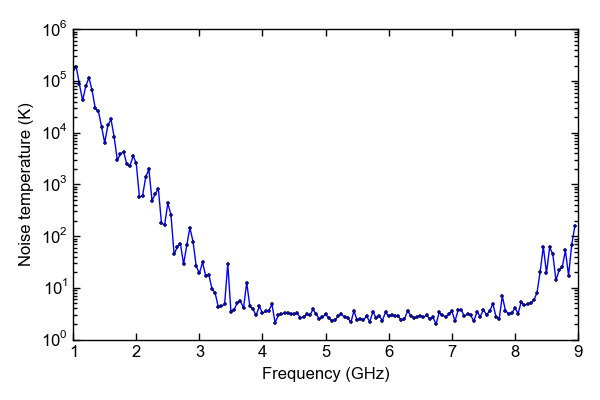
\includegraphics[width = .7 \linewidth]{Figures/Noise/noise_temperature_versus_power.png}
    \caption{Noise temperature versus frequency. The noise temperature has been calculated for $160$ frequencies in the range \SIrange{1}{9}{\giga \hertz}. For each frequency $2001$ points were measured, from which the signal, noise, SNR, and noise temperature was determined. Measurements were performed at an input power of \SI{-113}{\dBm} and an IF bandwidth of $\Delta f = $\SI{300}{\hertz}.}
    \label{fig:Noise temperature}
\end{figure}

Using the Rhode \& Schwarz ZVM vector network analyzer, The transmission has been measured for $160$ equidistant frequencies in the range \SIrange{1}{9}{\giga \hertz}. For each frequency a total of $2001$ points was measured with an IF bandwidth $\Delta f = $ \SI{300}{\hertz}. From these measurements the signal-to-noise ratio has been determined for each frequency. With knowledge of the SNR, the noise temperature has then been determined as a function of frequency using Equation~\ref{eqn:noise temperature} . The result is shown in Figure~\ref{fig:Noise temperature}.

From Figure~\ref{fig:Noise temperature} it is clear that the noise temperature is highly temperature-dependent. In the frequency range \SIrange{4}{8}{\giga \hertz} the noise temperature is quite low, never reaching above \SI{10}{\kelvin}. This is exactly the bandwidth of the cryogenic low-noise amplifier by Low Noise Factory, which is the first amplifier in the amplification chain. From the specifications of the amplifier, the noise temperature of the amplifier has been calculated at an ambient temperature of \SI{8}{\kelvin}, and equals roughly \SI{4}{\kelvin} for the entire bandwidth. Comparing the amplifier specifications with Figure~\ref{fig:Noise temperature}, it is likely that in the frequency range \SIrange{4}{8}{\giga \hertz} the first amplifier is the component contributing most to the total noise temperature.

Outside the \SIrange{4}{8}{\giga \hertz} frequency band, however, the noise temperature rapidly increases. This is partly due to the frequency lying outside of the bandwidth of the amplifier, in which case the amplification will be lower. However, this is not an adequate explanation for the fact that the noise temperature increases to several hundred thousand Kelvin. The reason for this unrealistic noise temperature is that in our model we did not take into account the noise added by components after the amplifier. While the gain of the amplifier decreases outside its bandwidth, the components after the amplification will still add the same amount of noise. When the gain decreases by a significant amount, the relative contribution of these post-amplification noise sources will increase. Furthermore the assumption that the noise spectrum is white is no longer correct at low frequencies, where $1/f$ noise starts to contribute.

\begin{figure}[h]
    \centering
    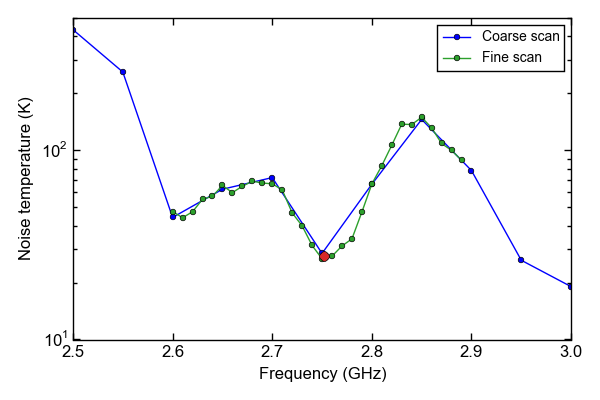
\includegraphics[width = .6\linewidth]{Figures/Noise/noise_temperature_versus_power_detailed.png}
    \caption{Detailed scan of noise temperature versus frequency in the range \SIrange{2.6}{2.9}{\giga \hertz}. The resonator with $f_0 = $\SI{2.75}{\giga \hertz} (red dot) seems to reside at a local minimum of the noise temperature.}
    \label{fig:noise temperature 2GHz}
\end{figure}

From Figure~\ref{fig:Noise temperature} it can be seen that the noise temperature can vary by a large amount between consecutive points. To determine whether this variation is due to a large uncertainty, or due to the noise temperature actually fluctuating strongly with varying frequency, a more detailed scan has been performed in the frequency region \SIrange{2.6}{2.9}{\giga \hertz}, in which one resonator has a resonance frequency. The result is shown in Figure~\ref{fig:noise temperature 2GHz}. As the curve of the detailed scan follows the curve of the coarse scan pretty closely, it can be concluded that the noise temperature of the system in fact fluctuates quite strongly with varying frequency.

Another point of interest is that the resonance frequency of the resonator lies near the local minimum of the noise temperature in that region. This is quite a stroke of luck, as a slightly higher or lower frequency would have resulted in a much higher noise temperature.



\section{Conclusion and future work}

The noise temperature gives us an estimate of the noise added to the system. It has been shown that the noise temperature can fluctuate strongly with varying frequency. In the model used to estimate the noise temperature it has been shown that outside the bandwidth of the amplifier the model breaks down. At this point the noise added by the components after the amplification, and indeed even the amplifiers themselves, needs to be taken into account to obtain accurate estimates of the noise temperature.

However, even outside of the bandwidth of the amplifier, there are frequency regions in which the noise temperature may still be acceptable. It is therefore a good idea to initially perform measurements of the noise temperature of the set-up. This will give an indication of the signal-to-noise ratio, from which accurate estimates can be made as to what the amount of measurement time is needed to obtain a desired SNR.

The noise temperature measurements were performed using the Rhode \& Schwarz ZVM vector network analyzer. It would be interesting to see how other measurement set-ups would compare to the vector network analyzer. One interesting candidate would be a heterodyne detector. However, as the vector network analyzer can also measure phase, a fair comparison would also require the heterodyne detector to be able to measure the phase. This heterodyne detector is currently being set up, and will hopefully soon yield interesting results.

Aside from only comparing the noise temperature, other properties are also important when comparing two set-ups. One of these is the duty cycle, which is the percentage of time acually spent measuring. For the vector network analyser the duty cycle seems to be around $50\%$, provided that a single measurement sweep takes at least a few seconds. Other set-ups may therefore offer an improvement in the duty cycle. Furthermore, properties such as phase stability and uncertainty would also be interesting to compare.

Another interesting measurement would be to see if the noise temperature as a function of frequency remains the same in future cooldowns, and for different samples.



\externaldocument[A-]{Chapters/DRIE.tex}
\externaldocument[A-]{Chapters/Muxmon.tex}

\chapter{Photon number calculation}
  \label{ch:photon number calculation}

  In cQED resonators usually operate in the single-photon regime. It is therefore important to know what power is required to reach this regime. In the equilibrium state of the resonator the power absorbed $P_\text{abs}$ by the resonator is equal to the power leaking out of the resonator, and so the absorbed power $P_\text{abs}$ can be expressed as:

  \begin{equation}
    P_\text{abs} = \left<n_\text{ph}\right>\hbar\omega_r \kappa
    \label{eq:Pabs-nph}
  \end{equation}

  where $\kappa=\omega_r/Q_i$ is the cavity decay rate.

  The absorbed power $P_\text{abs}$ can also be expressed in terms of the input power $P_\text{in}$ entering the feedline. We note that the absorbed power $P_\text{abs}$ is equal to the input power $\P_\text{in}$ entering the feedline minus the reflected power $P_\text{refl}$ and the transmitted power $P_\text{trans}$. These are given by:

  \begin{align}
    P_\text{refl} = P_\text{in}\left|S_{11}\right|^2\\
    P_\text{trans} = P_\text{in}\left|S_{21}\right|^2\\
  \end{align}

  where $S_{11}$ and $S_{21}$ are the scattering parameters. At the resonance frequency $S_{21}=\frac{Q_c}{Q_i+Q_c}$ (see Eq.~\ref{eq:S21min}), and $S_{11}=S_{21}-1$. Therefore the absorbed power is equal to:

  \begin{equation}
    P_\text{abs}=1-P_\text{refl}-P_\text{trans}=\frac{2Q_l^2}{Q_c Q_i}P_\text{in}
    \label{Pabs-Pin}
  \end{equation}

  Combining Eqs.~\ref{eq:Pabs-nph} and~\ref{Pabs-Pin}, we arrive at a formula for the mean photon number $\left<n_\text{ph}\right>$:

  \begin{equation}
    \left<n_\text{ph}\right> = \frac{2}{\hbar \omega_r}\frac{Q_l^2}{Q_c}P_\text{in}
  \end{equation}

  The input power $P_\text{in}$ can be found by measuring the transmission of the components between the generator and feedline.



\chapter{Duplexer isolation}
  \label{ch:Duplexer isolation}

  \begin{figure}[h]
    \centering
    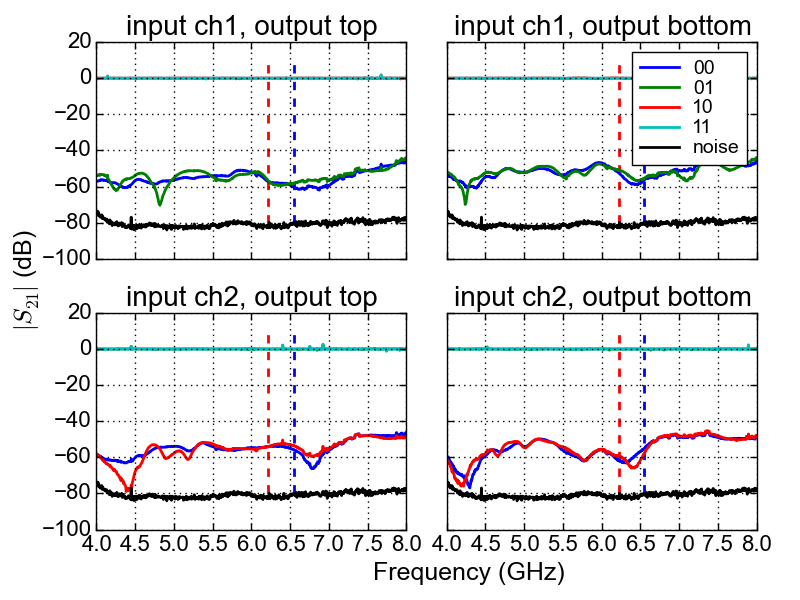
\includegraphics[width=\textwidth]{Figures/Appendix/Duplexer isolation.png}
    \caption{Isolation of the Duplexer. Legend indices correspond to switch state($1$ means open, $0$ means closed, lsb corresponds to bottom drive line, msb to top drive line). Transmission is measured relative to transmission when all channels are open (11). The black line corresponds to the measured noise floor. The red dashed line indicates the frequency of the top and bottom qubit, and the blue dashed line to the ancilla qubit, during the Muxmon experiment.}
    \label{fig:Duplexer isolation}
  \end{figure}

  The isolation of the Duplexer switches has been measured. During the measurements a signal was sent through input channel $1$ and $2$, corresponding to the signal of the main Gaussian pulse, and derivative pulse, respectively. For each input channel the transmission to each of the two output channels has been measured. These output channels are connected to the drive lines of the top and bottom qubit during the Muxmon experiment. For each input-output port combination the transmission has been measured for different switch configurations, which were controlled using the nanosecond-switches. Four different switch combinations were used, corresponding the the four distinct possibilities of the signal being directed to each of the two output channels.

  The results of the isolation measurements are shown in Fig.~\ref{fig:Duplexer isolation}. As can be seen in all four input-output combinations the isolation is around \SI{50}{\dBm} at the frequency of top and bottom qubit. Furthermore, the isolation does not seem to depend strongly on whether the switch to the other output port is open or closed.

\chapter{Chip characterization}

  \section{Muxmon1 cross-driving}
    \label{sec:Muxmon1 cross-driving}
      \begin{table}[h]
        \begin{tabular}{l c c}
          \toprule
          qubit & \multicolumn{2}{c}{cross-driving (\%)} \\
          \cmidrule(lr){2-3}
               & top-ancilla drive line & bottom-ancilla drive line \\
          \midrule
          Top     & $100$    & $5.22$ \\
          Ancilla & $75$ & $62.5$ \\
          Bottom  & $1.05$ & $100$    \\
          \bottomrule
        \end{tabular}
        \label{tab:Muxmon1 cross-driving}
      \end{table}

  \section{Muxmon0 resonator buses}
    \label{sec:Resonator buses}

    \begin{figure}[h]
      \centering
      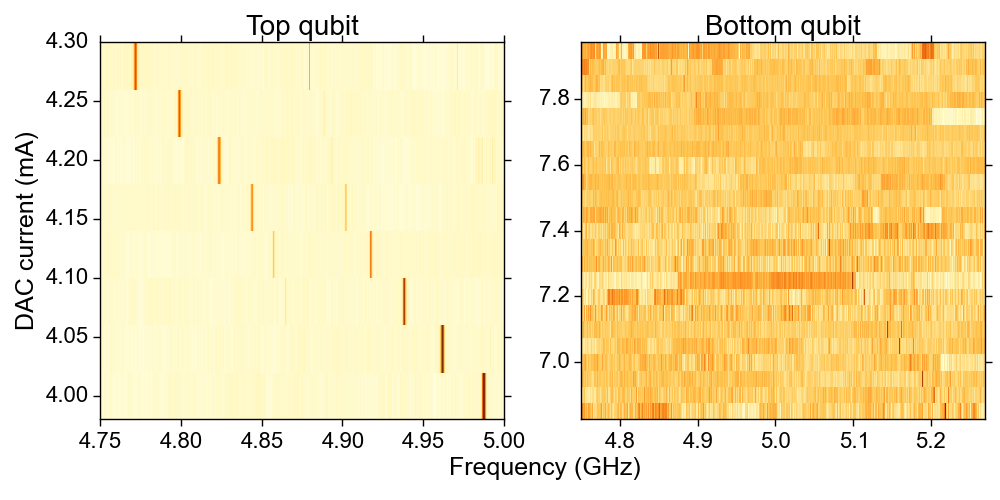
\includegraphics[width=\textwidth]{Figures/Appendix/resonator buses.png}
      \caption{Normalized transmission showing the resonator buses of the top and bottom qubit, at frequencies \SI{4.88}{\giga \hertz} and \SI{4.97}{\giga \hertz} respectively.}
      \label{fig:resonator buses}
    \end{figure}

    The top and bottom qubit are each coupled to a resonator bus. When the frequency of a qubit approaches that of the bus, they experience an avoided crossing. In Fig.~\ref{fig:resonator buses} these avoided crossing are shown for the top and bottom qubit. For the top qubit the frequency of the resonator bus is found to be \SI{4.88}{\giga \hertz}. For the bottom qubit the signal was considerably worse, but the frequency of the resonator bus is found to be roughly \SI{4.97}{\giga \hertz}. For the top qubit the coupling strength $g$ between the qubit and the bus can be extracted. It is equal to half the minimum distance, and approximately equal to \SI{27}{\mega \hertz}.

\chapter{Additional notes}
  \section{Qubit characterization}
      \subsection{Finding the qubit sweet-spot using a one-dimensional scan}
        \label{Finding the qubit sweet-spot using a one-dimensional scan}
        \begin{figure}[tb]
          \centering
          \includegraphics[width=.6\linewidth]{Figures/Qubit characterization/Resonator vs DAC linecut.png}
          \caption{Fixed frequency transmission versus DAC current. The frequency is chosen to be slightly below the resonator frequency found when the DAC current is set to zero. The symmetry point in the linecut corresponds to the sweet-spot of the ancilla qubit.}
          \label{fig:resonator vs dac linecut}
        \end{figure}

        As explained in Sec.~\ref{Scan for qubit sweet-spots}, the sweet-spot of a qubit can be found by performing a series of resonator scans while varying the DAC current. There is however, a faster approach for finding the qubit sweet-spot, at the cost of providing less information. This is done by choosing a fixed frequency close to the resonator's frequency $\wres$ (preferably slightly below, where the transmission slope is steepest). By measuring the amount of transmission as the DAC voltage is being varied, one obtains essentially a line-cut of the 2D scan. The idea this measurement is that if the qubit frequency $\fqub$ decreases, so does resonator frequency, resulting in a decrease in transmission (closer to $\wres$). Likewise, if the qubit frequency $\wqub$ increases, so does the resonator frequency, resulting in an increase in transmission (further away from $\wres$).

        At the qubit's sweet-spot, the resonator's frequency $\wres$ is at a maximum, and so the transmission should also be at a maximum. Furthermore, because the qubit frequency is symmetric with respect to its sweet-spot, so should the transmission. The sweet-spot can therefore be determined by finding the symmetric point in the transmission. In Fig.~\ref{fig:resonator vs dac linecut} one such linecut is shown. The transmission is clearly symmetric, and the symmetric point is equal to the qubit sweet-spot.

        If the resonator's frequency $\wres$ shifts by a large amount in the course of this measurement, it becomes harder to determine where the sweet-spot is (although even then often it can still be discerned). Nevertheless, this method is considerably faster than performing a full two-dimensional scan of frequency versus DAC voltage, and in most cases does provide sufficient information to determine the sweet-spot.


      \subsubsection{Spectroscopy}
        \begin{itemize}
          \item If the deviation in transmission becomes less due to more detuning, increasing the power can also increase the contrast.
        \end{itemize}
      \subsubsection{Flux matrix}
        After determining the flux matrix $\boldsymbol{F}$, there will still be some small remaining cross-coupling, which depends on the accuracy of the measurements. The process of creating a flux matrix can then be repeated, but instead of using DAC voltages as the varying parameters to construct matrix $\boldsymbol{M}$, the virtual fluxes should be used. Furthermore, as the cross-coupling is small compared to before, the flux range can be much greater, such that small slopes can be accurately measured. The resulting flux matrix $\boldsymbol{F}_2$ can then simply be multiplied with the first flux matrix $\boldsymbol{F}$ to obtain a more accurate final flux matrix.
    \chapter{AllXY pulse sequence}
      \label{ch:AllXY pulse table}

      \begin{table}[h]
        \centering
        \begin{tabular}{c c c c }
          \toprule
          number & ideal $\left<z\right>$ & First pulse & Second pulse \\
          \midrule
          1  & 1  & $I$         & $I$         \\
          2  & 1  & $X_\pi$     & $X_\pi$     \\
          3  & 1  & $Y_\pi$     & $Y_\pi$     \\
          4  & 1  & $X_\pi$     & $Y_\pi$     \\
          5  & 1  & $Y_\pi$     & $X_\pi$     \\
          6  & 0  & $X_{\pi/2}$ & $I$         \\
          7  & 0  & $Y_{\pi/2}$ & $I$         \\
          8  & 0  & $X_{\pi/2}$ & $Y_{\pi/2}$ \\
          9  & 0  & $Y_{\pi/2}$ & $X_{\pi/2}$ \\
          10 & 0  & $X_{\pi/2}$ & $Y_\pi$     \\
          11 & 0  & $Y_{\pi/2}$ & $X_\pi$     \\
          12 & 0  & $Y_\pi$     & $Y_{\pi/2}$ \\
          13 & 0  & $X_\pi$     & $X_{\pi/2}$ \\
          14 & 0  & $X_{\pi/2}$ & $X_\pi$     \\
          15 & 0  & $X_\pi$     & $X_{\pi/2}$ \\
          16 & 0  & $Y_{\pi/2}$ & $Y_\pi$     \\
          17 & 0  & $Y_\pi$     & $Y_{\pi/2}$ \\
          18 & -1 & $X_\pi$     & $I$         \\
          19 & -1 & $Y_\pi$     & $I$         \\
          20 & -1 & $X_{\pi/2}$ & $X_{\pi/2}$ \\
          21 & -1 & $Y_{\pi/2}$ & $Y_{\pi/2}$ \\
          \bottomrule
        \end{tabular}
        \caption{The 21 pulses that comprises the AllXY pulse sequence.}
        \label{tab:AllXY sequence}
      \end{table}

      In Table~\ref{tab:AllXY sequence} the 21 pulse combinations are shown that comprise the AllXY pulse sequence. The AllXY measurement is able to diagnose specific sources contributing to gate errors (see Sec.~\ref{ssec:AllXY}). For a more detailed analysis on the AllXY see Reed's thesis~\cite{Reed}.

  \chapter{Randomized benchmarking}
    \section{Clifford gate decomposition}
      \label{ssec:Clifford gate decomposition}


        \begin{tabular}{c c c }
          \toprule
          Clifford nbr     & gate decomposition & \begin{tabular}{@{}c@{}}5 primitives decomposition \\\noalign{\smallskip} $X_{\pi/2} \quad Y_{\pi/2} \quad X_{\pi/2} \quad X_{-\pi} \quad Y_{-\pi}$ \end{tabular}\\
          \midrule
          1 & $ I$ & 0\quad\quad\;0\quad\quad\;0\quad\quad\;0\quad\quad\;0 \\
          2 & $ Y_{\pi/2} -  X_{\pi/2}$ & 0\quad\quad\;1\quad\quad\;1\quad\quad\;0\quad\quad\;0 \\
          3 & $ X_{-\pi/2} -  Y_{-\pi/2}$ & 1\quad\quad\;1\quad\quad\;0\quad\quad\;1\quad\quad\;0 \\
          4 & $ X_\pi$ & 0\quad\quad\;0\quad\quad\;0\quad\quad\;1\quad\quad\;0 \\
          5 & $ Y_{-\pi/2} -  X_{-\pi/2}$ & 0\quad\quad\;1\quad\quad\;1\quad\quad\;0\quad\quad\;1 \\
          6 & $ X_{\pi/2} -  Y_{-\pi/2}$ & 1\quad\quad\;1\quad\quad\;0\quad\quad\;0\quad\quad\;1 \\
          7 & $ Y_\pi$ & 0\quad\quad\;0\quad\quad\;0\quad\quad\;0\quad\quad\;1 \\
          8 & $ Y_{-\pi/2} -  X_{\pi/2}$ & 0\quad\quad\;1\quad\quad\;1\quad\quad\;1\quad\quad\;1 \\
          9 & $ X_{\pi/2} -  Y_{\pi/2}$ & 1\quad\quad\;1\quad\quad\;0\quad\quad\;0\quad\quad\;0 \\
          10 & $ X_\pi -  Y_\pi$ & 0\quad\quad\;0\quad\quad\;0\quad\quad\;1\quad\quad\;1 \\
          11 & $ Y_{\pi/2} -  X_{-\pi/2}$ & 0\quad\quad\;1\quad\quad\;1\quad\quad\;1\quad\quad\;0 \\
          12 & $ X_{-\pi/2} -  Y_{\pi/2}$ & 1\quad\quad\;1\quad\quad\;0\quad\quad\;1\quad\quad\;1 \\
          13 & $ Y_{\pi/2} -  X_\pi$ & 0\quad\quad\;1\quad\quad\;0\quad\quad\;1\quad\quad\;0 \\
          14 & $ X_{-\pi/2}$ & 0\quad\quad\;0\quad\quad\;1\quad\quad\;1\quad\quad\;0 \\
          15 & $ X_{\pi/2} -  Y_{-\pi/2} -  X_{-\pi/2}$ & 1\quad\quad\;1\quad\quad\;1\quad\quad\;0\quad\quad\;1 \\
          16 & $ Y_{-\pi/2}$ & 0\quad\quad\;1\quad\quad\;0\quad\quad\;0\quad\quad\;1 \\
          17 & $ X_{\pi/2}$ & 0\quad\quad\;0\quad\quad\;1\quad\quad\;0\quad\quad\;0 \\
          18 & $ X_{\pi/2} -  Y_{\pi/2} -  X_{\pi/2}$ & 1\quad\quad\;1\quad\quad\;1\quad\quad\;0\quad\quad\;0 \\
          19 & $ Y_{-\pi/2} -  X_\pi$ & 0\quad\quad\;1\quad\quad\;0\quad\quad\;1\quad\quad\;1 \\
          20 & $ X_{\pi/2} -  Y_\pi$ & 1\quad\quad\;0\quad\quad\;0\quad\quad\;0\quad\quad\;1 \\
          21 & $ X_{\pi/2} -  Y_{-\pi/2} -  X_{\pi/2}$ & 1\quad\quad\;1\quad\quad\;1\quad\quad\;1\quad\quad\;1 \\
          22 & $ Y_{\pi/2}$ & 0\quad\quad\;1\quad\quad\;0\quad\quad\;0\quad\quad\;0 \\
          23 & $ X_{-\pi/2} -  Y_\pi$ & 1\quad\quad\;0\quad\quad\;0\quad\quad\;1\quad\quad\;1 \\
          24 & $ X_{\pi/2} -  Y_{\pi/2} -  X_{-\pi/2}$ & 1\quad\quad\;1\quad\quad\;1\quad\quad\;1\quad\quad\;0 \\
          \bottomrule
        \end{tabular}

      % \begin{figure}[tb]
      %   \centering
      %   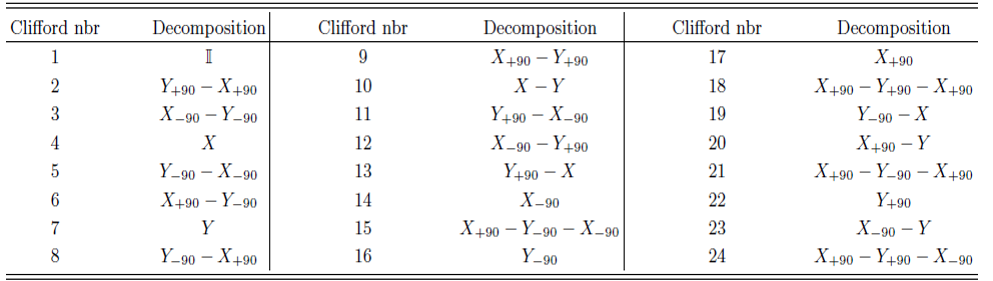
\includegraphics[width=\textwidth]{Figures/Clifford decomposition.png}
      %   \caption{Decomposition of all $24$ Cliffords into X and Y rotations}
      %   \label{fig:Clifford decomposition}
      % \end{figure}
      % \textbf{TODO:} Cite


    \section{Determining population in three states}
      \label{ssec:Determining population in three states}
      If there were no leakage present during randomized benchmarking, the full information about the state populations can be extracted from the randomized benchmarking results. However, if leakage to the second-excited state is present, the full information about the populations of the three states can be extracted using two versions of randomized benchmarking, one without a final pi pulse, and one with a final pi pulse. The final pi pulse swaps the populations in the ground and excited state. We assume that the population of the second excited-state remains unaffected by this single final pulse.

      Using these two randomized benchmarking sequences, two different signals $S_0$ and $S_1$ are measured, corresponding to a measurement without a final pi pulse, and a measurement with a final pi pulse, respectively. This leads to the following three equations:

      \begin{align}
        p_0 V_0 + p_1 V_1 + p_2 V_2 = & S_0 \notag\\
        p_1 V_1 + p_0 V_1 + p_2 V_2 = & S_1 \notag\\
        p_0 + p_1 + p_2 = &   1
        \label{eq:three populations equations App}
      \end{align}

      where $p_i$ corresponds to the final population in state $\ket{i}$, and $V_i$ is the signal of state $\ket{i}$.  Filling in $p_2 = 1 - p_0 - p_1$ into the first two equations of \ref{eq:three populations equations App}, we are left with the following set of equations:

      \begin{align}
        \begin{bmatrix}
          V_0 - V_2 & V_1 - V_2 \\
          V_1 - V_2 & V_0 - V_2
        \end{bmatrix}
        \begin{bmatrix}
          p_0 \\
          p_1
        \end{bmatrix}
        =
        \begin{bmatrix}
          S_0 - V_2 \\
          S_1 - V_2
        \end{bmatrix}
      \end{align}

      This set of equations can be easily solved by matrix inversion, resulting in the following three populations:

      \begin{align}
        \begin{bmatrix}
          p_0 \\
          p_1
        \end{bmatrix}
        = &
        \left((V_0-V_2)^2 - (V_1 - V_2)^2\right)^{-1}
        \begin{bmatrix}
          V_0 - V_2 & -V_1 + V_2 \\
          -V_1 + V_2 & V_0 + V_2
        \end{bmatrix}
        \begin{bmatrix}
          S_0 - V_2 \\
          S_1 - V_2
        \end{bmatrix} \notag\\
        p_2 = & 1 - p_0 - p_1
        \label{eq:RB populations using final pi}
      \end{align}
      If one has knowledge of all thee signals $V_0$, $V_1$ and $V_2$ (see Sec.~\ref{ssec:Second excited-state} for information on measuring $V_2$), the three populations can be obtained using Eq.~\ref{eq:RB populations using final pi}.
      \newpage
  \section{Two qubit randomized benchmarking leakage}
    \label{sec:Two qubit randomized benchmarking leakage}
        \begin{table}[h]
          \begin{tabular}{c c c c c}
            \toprule
            RB mode & \multicolumn{2}{c}{Top qubit} & \multicolumn{2}{c}{Bottom qubit} \\
            \cmidrule(lr){2-3}
            \cmidrule(lr){4-5}
            & $T_1^2 (\mu s)$ & $\alpha$ (\%) & $T_1^2$ $(\mu s)$ & $\alpha$ (\%) \\
            \midrule
            Alternating  & $10.0(6)$    & $0.027(1)$ & $4.9(1.9)$  & $0.011(5)$\\
            Compiled     & $8.8(6)$    & $0.024(1)$  & $4.5(9)$ & $0.011(2)$\\
            5 primitives &$9.7(7)$    & $0.038(3)$  & $4.9(1)$  & $0.018(5)$\\
            \bottomrule
          \end{tabular}
        \end{table}


        \begin{figure}[h]
          \centering
          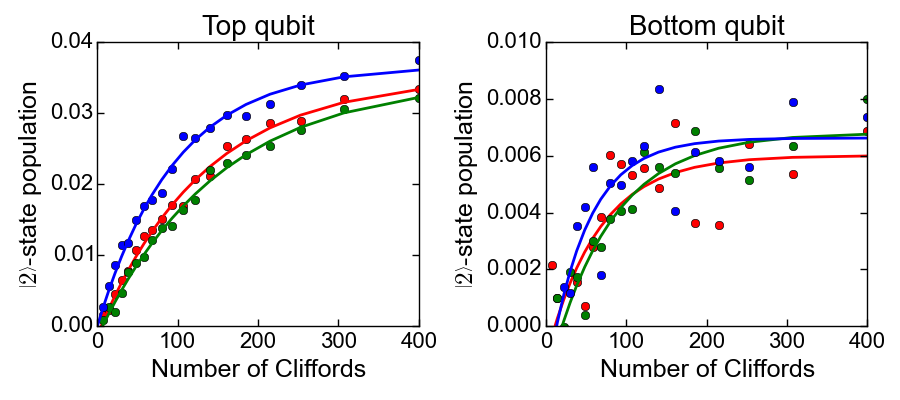
\includegraphics[width=\textwidth]{Figures/Randomized benchmarking/2nd-state leakage 2Q.png}
          \caption{Second state leakage along with fit using Eq.~\ref{eq:2nd state formula}.}
          \label{fig:second state leakage 2Q}
        \end{figure}

\chapter{Compiled randomized benchmarking algorithm}
  \label{sec:compiled randomized benchmarking algorithm}
  \section{Finding the optimal gate sequence}
    In compiled randomized benchmarking each set of Cliffords is compiled such that the total number of pulses sent is as small as possible. This is done by comparing all the possible decompositions for each Clifford in the set of Cliffords with each other, and determining the combination that results in the least amount of total pulses. The constraints are that pulses may not be applied simultaneously, but may be directed to either or both of the qubits.

    Given a tuple of Cliffords $\left(C_{\alpha_1}^1, \dots, C_{\alpha_n}^n\right)$, where $n$ is the number of qubits and $\alpha_i$ is the Clifford number for qubit $i$, a particular decomposition of the Cliffords is given by $\left(\left( G_1^1, ..., G_{m_1}^1 \right) , ..., \left(G_1^n, ..., G_{m_n}^n\right)\right)$, where $m_i$ is the number of gates in the decomposition of Clifford $C_{\alpha_i}^i$, and $G_j^i$ is gate $j$ of the Clifford decomposition of $C_i$. The algorithm used for finding the minimum number of gates for a particular tuple of Clifford decompositions is a recursive algorithm. The algorithm determines all possible ways in which the gates can be ordered, and finally chooses the sequence having the smallest length.

    To explain this algorithm, let us denote $\bm{\beta}=\left(\beta_1, \dots, \beta_n\right)$ as the indices of the next possible gates. The corresponding gates are given by $\bm{G_\bm{\beta}}=\left( G_{\beta_1}^1, \dots, G_{\beta_n}^n \right)$. If the indices where $\beta_i=m_i + 1$, there is no next gate, and so $G_{\beta_i}$ does not exist and should not be added to $\bm{G_\bm{\beta}}$.

    \begin{enumerate}
      \item Start with an empty sequence of gates $G_\text{seq}$ and gate indices $\bm{\beta} = \left(\beta_1, ..., \beta_n\right) = \left(1, ..., 1\right)$
      \item Determine the set of distinct gates in $G_{\bm{\beta}}$.
      \item For each gate $g$ in the set of distinct gates perform the following steps:
      \begin{enumerate}
        \item Append $g$ to $G_\text{seq}$.
        \item Determine all indices $i$ for which the next gate $G_{\beta_i}^i$ equals $g$.
        \item Copy gate indices $\bm{\beta}$ to $\bm{\beta}^\text{new}=\left(\beta_1^\text{new}, ..., \beta_n^\text{new}\right)=\left(\beta_1, ..., \beta_n\right)$.
        \item For all indices $i$ for which $G_{\beta_i}^i=g$, increase the gate index $\beta_i^\text{new} = \beta_i+1$.
        \item Go to step two using the new gate indices $\bm{\beta}^\text{new}$.
      \end{enumerate}
      \item If $G_{\bm{\beta}}$ is empty, then $G_\text{seq}$ is a particular sequence of pulses that would result in all Cliffords being applied.
      \item When all possible sequences are combined, choose the sequence with the minimum number of gates in $G_\text{seq}$
    \end{enumerate}

    This algorithm determines the least amount of gates necessary to perform all Cliffords in one particular tuple of decompositions. However, each Clifford has on average $38$ different decompositions, and so for $n$ qubits the total decomposition combinations is approximately$38^n$, meaning this algorithm would have to be repeated $38^n$ times to find the global minimum number of pulses to perform all Cliffords. And in fact this would only determine the optimal compilation for one particular set of Cliffords; to find the average gates per Clifford tuple one would have to perform this on all possible combinations of Cliffords and then determine the average gates per Clifford tuple. This problem therefore scales exponentially with the number of qubits, and would seem impossible for as few as $n=3$ qubits, as it would require $24^3*38^3=7.6*10^8$ different decomposition combinations. Nevertheless the average gates per Clifford has been calculated exactly for up to $n=5$ qubits. This has been done using several optimization methods, which will be discussed below.

  \section{Optimizing the gate compilation algorithm}
    \label{Optimizing the gate compilation algorithm}
    Determining the average gates per Clifford tuple for $n=5$ qubits would initially result in $6.3*10^{14}$ different combinations of Clifford decompositions. For each of these combinations the algorithm must find the least amount of gates necessary to perform all gates in that particular set of Clifford decompositions. It is clear that this is computationally not viable. Luckily several optimizations can be performed which can drastically reduce this number by many orders of magnitude. These optimizations will be discussed in this section.

    The first and simplest optimization is from the simple observation that the optimal gate compilation for a certain tuple of Cliffords $\left(C_{\alpha_1}^1, \dots, C_{\alpha_n}^n\right)$ is the same as any permutation of those Cliffords. Therefore we only have to determine the optimal compilations for the tuples $\left(C_{\beta_1}^1, \dots, C_{\beta_n}^n\right)$ where $\beta_1 \leq \beta_2 \leq \dots \leq \beta_n$. This already reduces the amount of calculations by an exponential amount (a factor $81$ times less computations when $n=5$.

    The second optimization is to keep track of the minimum number of gates so far found that can compile a given tuple of Cliffords. At each stage of the algorithm it checks if the gates that are so far in $G_\text{seq}$ plus all the distinct gates left in $G_{\bm{\beta}}$ is equal to or greater than the minimum number of gates found so far. If this is the case, it will know that it cannot find a better combination of gates using the sequence $G_\text{seq}$. It can therefore stop this sequence and start with the next sequence. The minimum number of gates can initially be placed at $5$ gates, as the $5$ primitives method proves that there is always a decomposition of an arbitrary number of Cliffords into $5$ gates. This optimization places an upper bound on the number of gates, and results in a massive decrease in computation time. This is especially the case because as the minimum number of gates decreases, so does the frequency at which the algorithm stops its current sequence increase.

    The third optimization relies on the fact that it is more likely that decompositions with fewer gates result in an optimal gate compilation. Therefore the decompositions of all Cliffords have been arranged in ascending number of gates. When comparing the decompositions of the Cliffords the first decompositions compared are those with the fewest gates. The probability of finding the optimal gate compilation is therefore high, and even if it did not find the optimal gate compilation, it is likely that the minimum gate length found so far will be low. This optimization is especially effective when combined with the second optimization.

    The fourth optimization places a lower bound on the number of gates. For a given tuple of Cliffords $\left(C_{\alpha_1}^1, \dots, C_{\alpha_n}^n\right)$, the lower bound is found by looking at the optimal lengths previously found for all $n-1$ Clifford subsets. This requires knowledge of the lengths of all the $n-1$ Cliffords. Since the length of the tuple of $n$ Cliffords can never be less than any of the lengths of the $n-1$ Clifford subsets, the maximum of these lengths therefore places a lower bound on the optimal number of gates. This means that if during the algorithm ever finds one sequence of gates for any tuple of decompositions whose length is equal to this lower bound, it will know it has found the optimal gate compilation for the tuple of Cliffords, and may abort all further search. This is in contrast to the second optimization, where an upper bound was found, in which case only the particular sequence of gates could be aborted. As the number of qubits increases, it becomes more and more likely that the lower bound is equal to five. In this case the lower bound is equal to the upper bound set by the $5$ primitives method, and so it can immediately be concluded that the optimal gate compilation is the $5$ primitives method. This optimization that places a lower bound is probably the best of all optimizations used, and results in a massive gain in computation time, by many orders of magnitude.

    The fifth optimization is the most complicated optimization, and is based on separating all decompositions with three gates or less from those composed of four gates. In this optimization first all combinations are tested using only decompositions with three or less gates. This greatly reduces the average number of decompositions per Clifford, from $38$ to $7$. Especially as the number of qubits increases, this results in drastically less comparisons in total. Now it is not always the case that the minimum number of gates is found using only up to three gates per decomposition: sometimes the optimal gate compilation requires one of the decompositions to have four gates. However, we only need to include four gate decompositions when the lower bound is four or less and when the minimum gate compilation found using only three gates or less is equal to five or more. Only in this case could there be a four gate decomposition that could outperform gate decompositions with only three gates or less. We furthermore know that if there is such a four gate decomposition that results in the optimal gate compilation, its length must be equal to four, as the $5$ primitives method places the upper bound at $5$ gates. We therefore also know that only one Clifford can have a four gate decomposition, and all other Cliffords must be subsets of these four gates. We can therefore simply loop over each of the four gate decompositions, and test whether all other Cliffords are subsets of these four gates. This changes the comparison from scaling exponential with the number of qubits to scaling linear with the number of qubits.

    \begin{table}
      \begin{tabular}{c c || c c}
        \toprule
        number of qubits  & average gates per Clifford & number of qubits  & average gates per Clifford \\
        \midrule
        1 & 1.875 & 6  & 4.380 (12)\\
        2 & 2.925 & 7  & 4.570 (15)\\
        3 & 3.521 & 8  & 4.721 (10)\\
        4 & 3.874 & 9  & 4.808 (14)\\
        5 & 4.137 & 10 & 4.857 (24)\\
        \bottomrule
      \end{tabular}
      \caption{The average gates per Clifford after compilation. Values up to n=5 have been calculated exact, while values starting from n=6 have been determined using random sampling.}
      \label{tab:gates per Clifford}
    \end{table}

    Using these $5$ optimizations the average gates per Clifford tuple has been calculated exactly for $n=5$ qubits within two hours. Furthermore, the average gates per Clifford has been approximated for up to $n=10$ Cliffords using random sampling. The results are shown in Table~\ref{tab:gates per Clifford}.
